\documentclass[french]{article}
\usepackage[T1]{fontenc}
\usepackage[utf8]{inputenc}
\usepackage{lmodern}
\usepackage{graphicx}
\usepackage[a4paper,left=3cm,right=3cm,top=2.5cm,bottom=2.5cm]{geometry}
\usepackage{babel}

\usepackage{fancyhdr}
\pagestyle{fancy}
\renewcommand{\headrulewidth}{1pt}
\fancyhead[L]{Algorithmique et Programmation Avancée}
\fancyfoot[R]{Ebersold, Thieblin, Desprat}
\fancyhead[R]{Département Mathématiques-Informatique}
\fancyfoot[L]{MIA0301V - MI00304}


\usepackage{listingsutf8}
\usepackage{listings}
\usepackage{xcolor}
\lstset { %
	language=C++,
    basicstyle=\footnotesize\ttfamily,
    keywordstyle=\color{blue}\ttfamily,
    stringstyle=\color{red}\ttfamily,
    commentstyle=\color{olive}\ttfamily,
    morecomment=[l][\color{magenta}]{\#},
	backgroundcolor=\color{black!5}, % set backgroundcolor
	numbers=left, 
    numberstyle=\tiny\ttfamily, 
    breaklines=true,
    numbersep=5pt,
    xleftmargin=.25in,
    xrightmargin=.25in
}
\lstset{%
	inputencoding=utf8,
	extendedchars=true,
	literate=%
	{é}{{\'e}}{1}%
	{è}{{\`e}}{1}%
	{à}{{\`a}}{1}%
	{ç}{{\c{c}}}{1}%
	{œ}{{\oe}}{1}%
	{ù}{{\`u}}{1}%
	{É}{{\'E}}{1}%
	{È}{{\`E}}{1}%
	{À}{{\`A}}{1}%
	{Ç}{{\c{C}}}{1}%
	{Œ}{{\OE}}{1}%
	{Ê}{{\^E}}{1}%
	{ê}{{\^e}}{1}%
	{î}{{\^i}}{1}%
	{ô}{{\^o}}{1}%
	{û}{{\^u}}{1}%
	{ë}{{\¨{e}}}1
	{û}{{\^{u}}}1
	{â}{{\^{a}}}1
	{Â}{{\^{A}}}1
	{Î}{{\^{I}}}1
}


\begin{document}
	
	\begin{minipage}{\textwidth}
		\begin{center}
			
			{\Large Mise en œuvre avec C++ \\ Feuille d'exercices : \textbf{les Piles}}
		\end{center}
	\end{minipage}
	\section{Implantez les opérations d’une pile spécifiées dans le cours}
On désire réaliser la notion de pile à l'aide d'une structure de données. 
Le type \texttt{Pile} est une structure de données comportant 2 \textbf{champs} :
\begin{description}
	\item[Elts] : tableau devant contenir les éléments de la pile. La capacité de la pile est définie par~\texttt{MAX}\footnote{En C++ pour définir une macro \texttt{NOMMACRO} associée à une valeur \texttt{MAVALEUR}, on utilise \texttt{\#define NOMMACRO MAVALEUR} -- i.e. à chaque fois qu'on utilise \texttt{NOMMACRO}, la valeur \texttt{MAVALEUR} associée sera utilisée. Ici, on s'en sert pour définir une constante \texttt{MAX} à 100}. Les éléments de ce tableau sont de type \textbf{entiers}.
	\item[NbElts] : nombre d’éléments dans la pile. On supposera que les éléments de la pile sont rangés dans l’ordre des indices croissants : le haut de la pile étant l'élément avec le plus grand indice du tableau. Pour une pile vide, NbElts doit être égal à zéro.
\end{description}

$\rightarrow$\textbf{Trouver les erreurs} le Listing \ref{list1} et \textbf{écrire} le code corrigé.
	\begin{lstlisting}[caption={A corriger: Structure Pile},label=list1]
#define MAX 100
Struc Pile{
	tableauChar Elts[MAX];
	entier NbElts
} 
\end{lstlisting}

	\begin{lstlisting}[caption={Squelette de Pile},label=list2]
//creation d'une pile vide initialisée
Pile initPile(){}
// le rajout d un élément se fait en fin de pile
void empiler(char element,Pile &p){} (/!\ MAX pile atteint)
// On peut vider la pile dans sa totalite
void purger(Pile &p){} 
//On supprime le dernier élément de la pile (/!\ pile vide)
bool depiler(Pile &p){}
// teste si la pile est vide
bool estVide(Pile &p){} 
// teste si la pile est pleine
bool estPleine(Pile &p){}
// retourne la longueur de la pile
int longueur(Pile &p){}
//retourne la valeur au sommet de la pile
int sommet(Pile &p){}
//fonction d'affichage
void afficherPile(Pile p){}
\end{lstlisting}
\begin{lstlisting}[caption={main a executer},label=list3]
int main(){
	Pile p = initPile();
	empiler(p,'a');
	empiler(p,'c');
	afficherPile(p);
	depiler(p);
	afficherPile(p);
	cin.get();
	return EXIT_SUCCESS;
}
\end{lstlisting}

\section{Ecrire un sous-programme vérifiant l’existence d’un élément de valeur << e >> dans la pile}

Ce traitement devra être basé sur une \textbf{recherche dichotomique}. Rappel: les caractères se comparent selon leur code ASCII : 0-9a-zA-Z 

\noindent\begin{minipage}{.65\textwidth}
	\begin{lstlisting}[caption={Recherche dichotomique dans un tableau trie}]
int rechercheDichotomique(Pile &pile, int val, int taille){
    int iDeb = //indice debut du tableau de debut de recherche
    int iFin = // indice du tableau de fin de recherche
    int iMil;// indice du tableau de milieu de recherche
    int index=-1;
    bool trouve = false;
    while( iDeb <= iFin && !trouve){
        //calcul de l'indice milieu
        //cas ou la valeur est au milieu
        //si ma valeur est avant le milieu, je cherche dans 1ere moitie
        //si ma valeur est apres le milieu, je cherche dans 2eme moitie
    }
    return index;
}
	\end{lstlisting}
\end{minipage}
\begin{minipage}{.45\textwidth}

		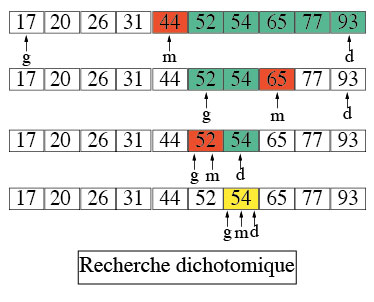
\includegraphics[width=0.9\textwidth]{dicho.jpg}

\end{minipage}\hfill


\section{Utilisation d’une pile : Application}
\textbf{Ecrire} un algorithme qui vérifie qu’un texte contenant des caractères standards est syntaxiquement correct du point de vue des parenthèses.

Les parenthèses sont de trois types : \texttt{ (, \{, [ } et leurs parenthèses fermantes correspondantes sont respectivement \texttt{), \}, ]}.
$\rightarrow$ on peut commencer juste par les parenthèses
\begin{lstlisting}[caption={Rappel : Déclaration d'une chaîne de caractères},label=stringrappel]
char x[] = "une chaine de caractères avec des parenthèses ())())))))(((())";
cout << x[0] << endl;//la console affiche : u
int tailleChaine= strlen(chaine); // recupere la taille de la chaine
cout << tailleChaine << endl;//la console affiche : 78
\end{lstlisting}

La correction syntaxique implique qu’à chaque parenthèse ouvrante corresponde une parenthèse fermante du même type, plus loin dans le texte.


Le texte compris entre ces deux parenthèses devra également être correct du point de vue des parenthèses.

\begin{lstlisting}[caption={Aide pour Verification syntaxe},label=aide]
//permet de verifier que les caracteres forment des paires ouvrantes et fermantes
bool sontDesPaires(char ouvrant,char fermant){
    //on verifie pour nos trois cas si le char ouvrant correspond bien au char fermant
}

bool verificationSyntaxe(char chaine[], Pile &pile){
    int tailleChaine= strlen(chaine); // recuperer la taille de la chaine passée en paramètre
    //parcours de la chaine de caractères
        //recupere le caratère courant
        //verifie si c'est un caractère spécial ouvrant
            //si oui, on ajoute ce caractere à la pile
            //sinon verifie si c'est un caractère spécial fermant
        
                //si oui verifie si la pile n'est pas vide
                //ou si le dernier caractère de la pile et le caractère courant forment une paire ouvrant/fermant
                    //si oui, on depile
                    //si non, ça veut dire que la chaine est mal formée
        
    //return : a la fin si la pile est vide ça indiquera que les paires sont bien formées, sinon qu'il y a eu une erreur
}
\end{lstlisting}

\begin{lstlisting}[caption={Exemple de main pour verifier la syntaxe},label=main]
int main(){
    char a[] = "()";
    char b[] = "(()";
    char c[] = "())";
    char d[] = "(())";
    char e[] = "une chaine de caractères avec des parenthèses ())())))))(((())";
    char f[] = "([{)";
    char g[] = "([{])";
    char h[] = "([{[()]}])";
    bool chaineValide=false;
    Pile p;
    p = initPile();
    chaineValide=verificationSyntaxe(a, p); // bien formé
    afficherResultat(chaineValide);
    chaineValide=verificationSyntaxe(b, p); //mal formé
    afficherResultat(chaineValide);
    //...
    
    cin.get();//attendre que l'utilisateur appuie sur ENTREE
    return 0;
}
\end{lstlisting}


\end{document}